\documentclass[journal,12pt,onecolumn]{IEEEtran}
\usepackage{mathtools,amssymb,amsfonts}
\usepackage{algorithmic}
\usepackage{algorithm}
\usepackage{graphicx}
\usepackage{xcolor}
\usepackage{float}
\usepackage{setspace}
\usepackage{subcaption}
\usepackage[hidelinks]{hyperref}
\usepackage{multirow}

\doublespacing

\hypersetup{
   colorlinks=true,
   linkcolor=blue,
   citecolor=black,
   urlcolor=blue
}

\usepackage{titlesec}
\titlespacing*{\section}{0pt}{12pt plus 4pt minus 2pt}{12pt plus 2pt minus 2pt}
\titlespacing*{\subsection}{0pt}{12pt plus 4pt minus 2pt}{8pt plus 2pt minus 2pt}
\titlespacing*{\subsubsection}{0pt}{12pt plus 4pt minus 2pt}{6pt plus 2pt minus 2pt}

\title{Genetic Algorithm: Bin Packing Problem}
\author{
   \IEEEauthorblockN{Matthew D. Branson} \\
   \IEEEauthorblockA{\textit{Department of Computer Science} \\
   \textit{Missouri State University}\\
   Springfield, MO \\
   branson773@live.missouristate.edu
   }
}

\date{July 5, 2025}

\begin{document}

\maketitle

\begin{abstract}
This paper presents the implementation and analysis of a...
\end{abstract}

\begin{IEEEkeywords}
Genetic Algorithms, Bin Packing Problem, Optimization, Heuristic Search
\end{IEEEkeywords}

\section{Q1: Encoding and Initialization}

An integer-based representation is used to encode bin assignments. For an instance with $N$ items, each individual is a vector of length $N$, where the value at index $i$ denotes the bin to which item $i$ is assigned.

For example, the encoding \texttt{[0, 1, 0, 2, 1, 1, 2, 1, 3, 0]} represents a solution for 10 items in which items 0, 2, and 9 are assigned to bin 0; items 1, 4, 5, and 7 to bin 1; items 3 and 6 to bin 2; and item 8 to bin 3, resulting in the use of 4 unique bins.

Initial populations are generated by assigning each item independently to a random bin in the range $[0, N-1]$. This produces diverse initial solutions while satisfying the constraint that the maximum number of bins does not exceed the number of items.

\section{Q2: Function Evaluation}

\subsection{Objective Function}

The objective function $f$ measures the number of unique bins used in a given individual. For instance, the encoding \texttt{[0, 1, 0, 2, 1, 1, 2, 1, 3, 0]} uses bins \{0, 1, 2, 3\}, yielding $f = 4$. The algorithm minimizes $f$ to reduce the total number of shipping boxes required.

\subsection{Constraint Handling}

The constraint violation function $g$ counts the number of bins whose total weight exceeds the 10 kg capacity. For each bin, the weights of assigned items are summed. A bin contributes 1 to $g$ if its cumulative weight exceeds the limit. A solution is considered feasible when $g = 0$.

\subsection{Evaluation Function}

Each individual is evaluated as a tuple $(f, g)$, where $f$ represents the number of bins used and $g$ the number of constraint violations. This formulation enables the algorithm to balance minimization of bin usage with satisfaction of feasibility constraints.


\section{Q3: GA Operations}

\subsection{Tournament Selection}

Tournament selection is used to construct a mating pool of $N$ individuals. For each selection, two candidates are drawn at random, and the winner is determined by a constraint-aware comparison rule. This process is repeated $N$ times. Mating pairs are then selected at random from the resulting pool.

\subsection{Winner Selection Rules}

Selection is guided by the following criteria:
\begin{itemize}
    \item If both individuals are feasible ($g_1 = 0$, $g_2 = 0$), the one with lower $f$ is preferred.
    \item If only one is feasible, the feasible individual is selected.
    \item If both are infeasible, the one with fewer violations ($g$) is selected.
\end{itemize}

These rules guide selection toward feasible individuals with fewer bins and penalize constraint violations when feasibility is not yet achieved.

\subsection{Crossover}

Two-point crossover is applied with a probability of 0.9. Two cut points are chosen to divide each parent chromosome into three segments. Offspring are generated by exchanging the middle segments, preserving the integer-based encoding and promoting genetic diversity.

\subsection{Mutation}

Each gene (bin assignment) is mutated independently with probability $p_m = 1/N$, where $N$ is the number of items. When selected, a gene is reassigned to a random integer in $[0, N-1]$. This maintains valid encodings while introducing variation for local exploration.

\section{Q4: GA Execution}

\subsection{Baseline Configuration}

The genetic algorithm was initially executed using the specified baseline parameters: population size of 20 and 50 generations. This configuration was tested on four problem instances containing 10, 25, 50, and 100 orders, with order weights uniformly distributed between 0 and 2 kg and a bin capacity of 10 kg.

\subsection{Parameter Variation Study}

To assess the impact of population size and generation count on performance, additional configurations were tested. Population sizes of 10 and 40 individuals were compared against the baseline of 20, while generation counts of 25 and 100 were compared against the baseline of 50. Additionally, each configuration was evaluated across all four problem sizes using three random seeds (42, 773, 2025) to examine performance variability.

\subsection{Fitness Plots}

The evolution of best and average fitness values across generations is shown for various configurations.

% Baseline configuration
\begin{figure}[htbp]
\begin{minipage}{0.48\textwidth}
    \centering
    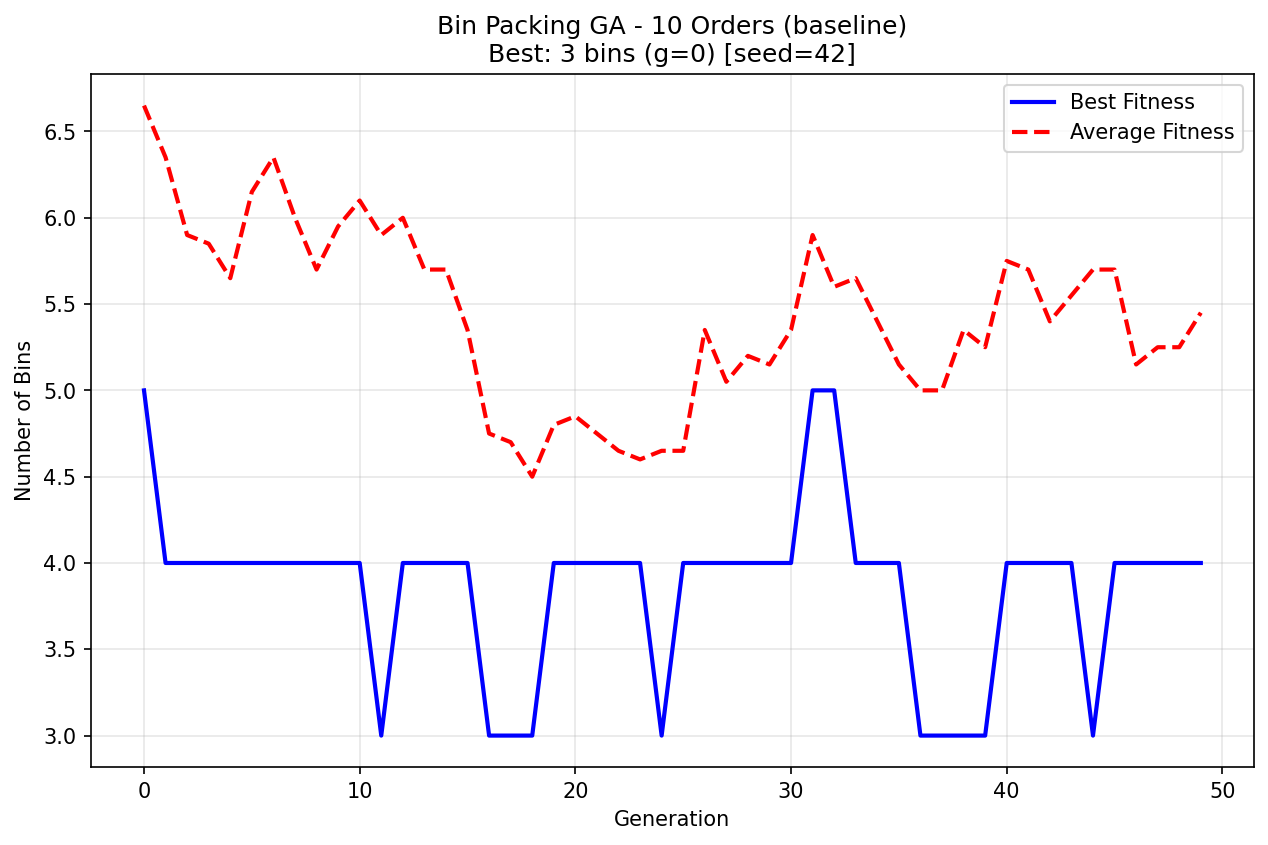
\includegraphics[width=\textwidth]{bpp_10items_baseline_seed42.png}
    \caption{Baseline: 10 orders}
    \label{fig:baseline_10}
\end{minipage}\hfill
\begin{minipage}{0.48\textwidth}
    \centering
    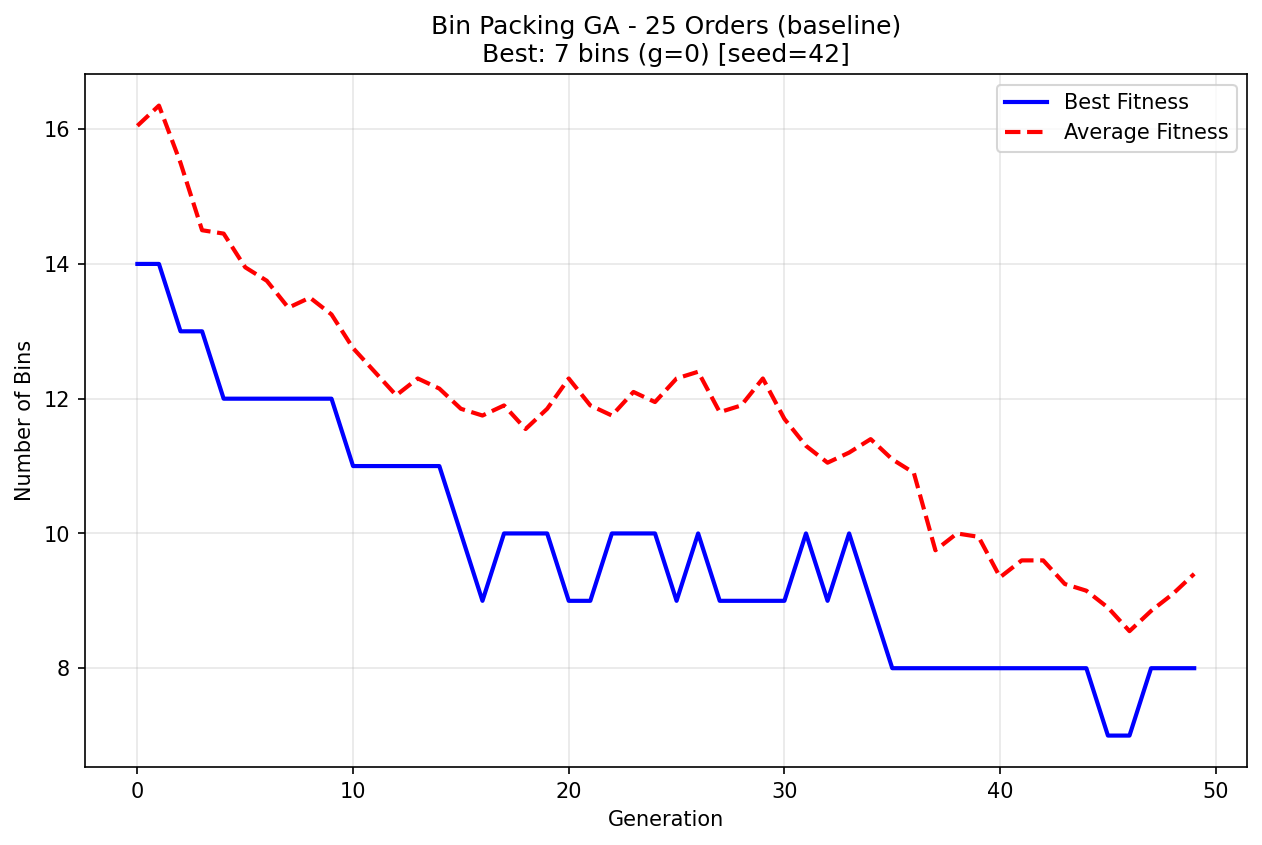
\includegraphics[width=\textwidth]{bpp_25items_baseline_seed42.png}
    \caption{Baseline: 25 orders}
    \label{fig:baseline_25}
\end{minipage}
\end{figure}

\begin{figure}[htbp]
\begin{minipage}{0.48\textwidth}
    \centering
    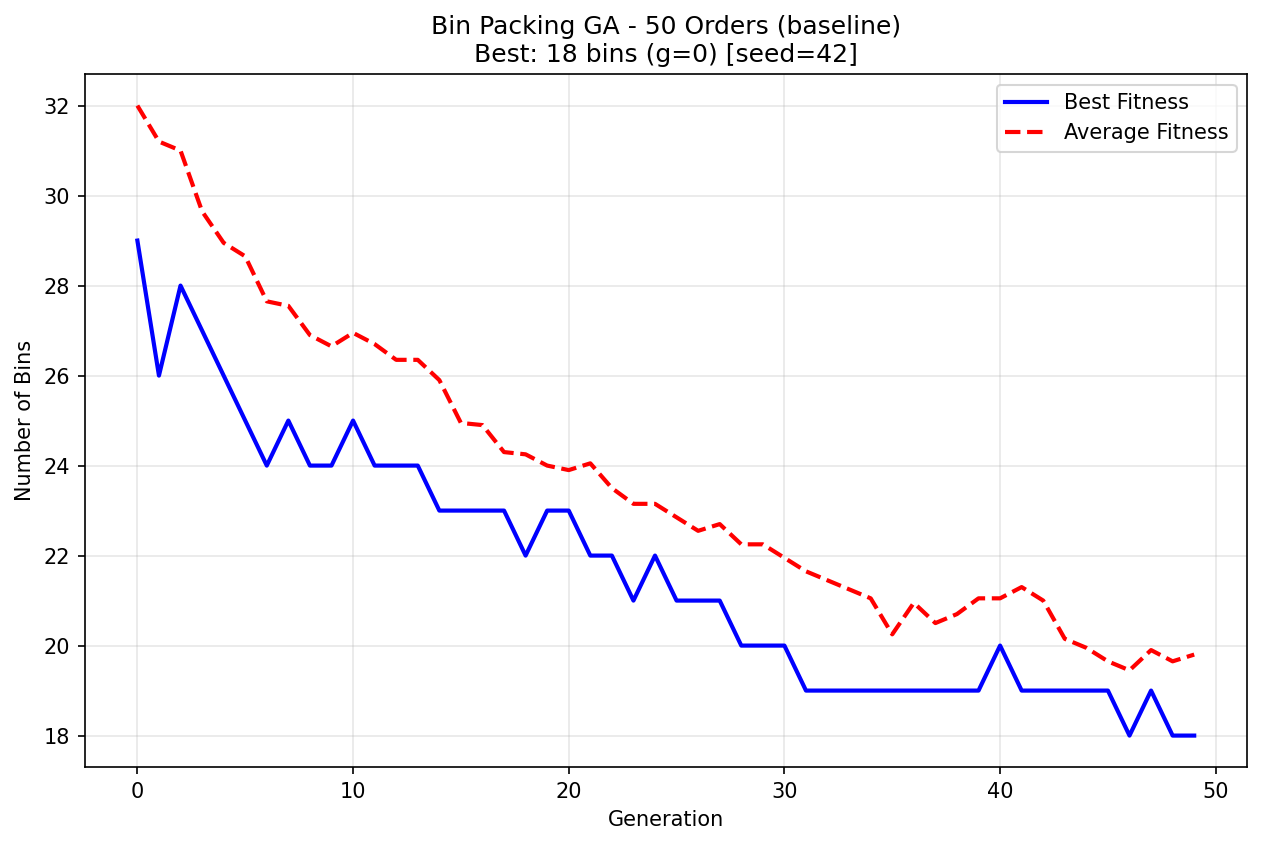
\includegraphics[width=\textwidth]{bpp_50items_baseline_seed42.png}
    \caption{Baseline: 50 orders}
    \label{fig:baseline_50}
\end{minipage}\hfill
\begin{minipage}{0.48\textwidth}
    \centering
    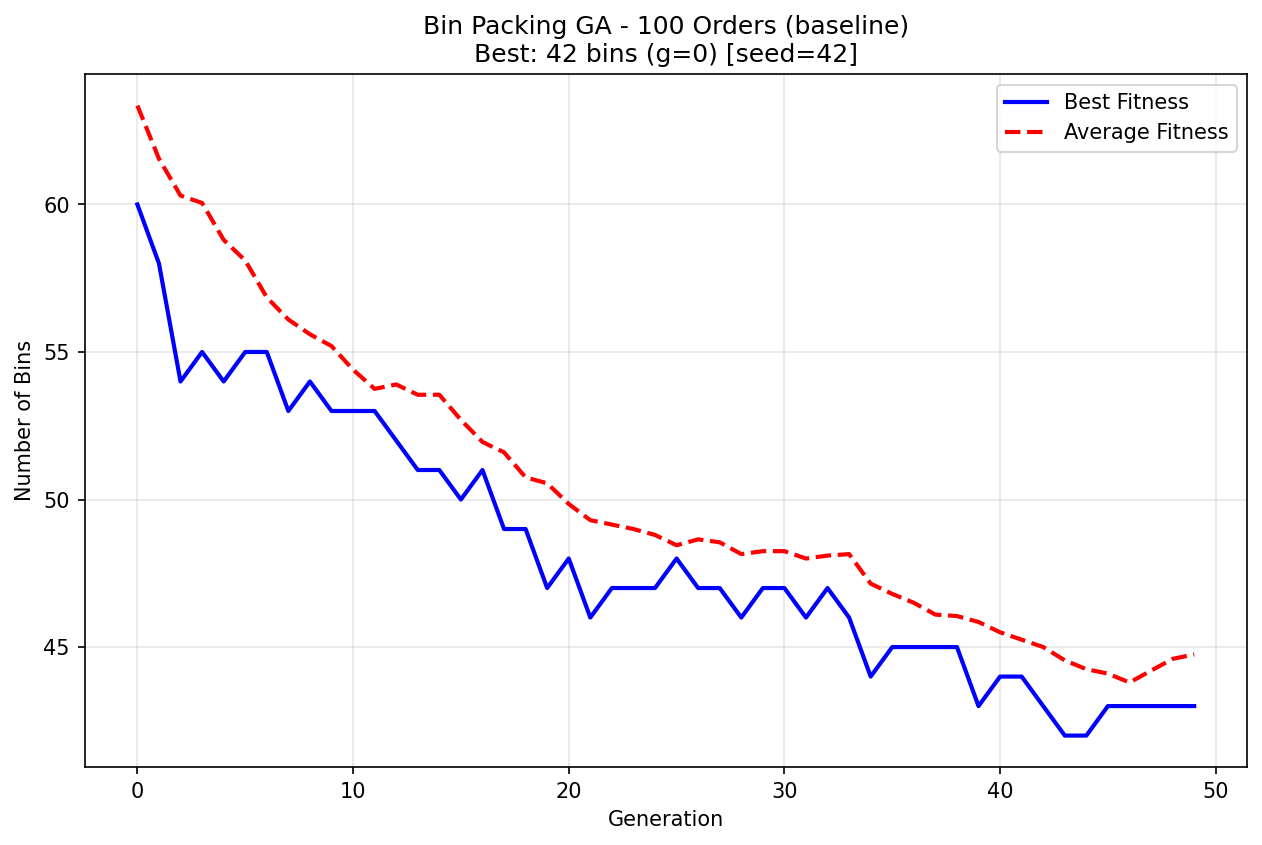
\includegraphics[width=\textwidth]{bpp_100items_baseline_seed42.png}
    \caption{Baseline: 100 orders}
    \label{fig:baseline_100}
\end{minipage}
\end{figure}

% Small population
\begin{figure}[htbp]
\begin{minipage}{0.48\textwidth}
    \centering
    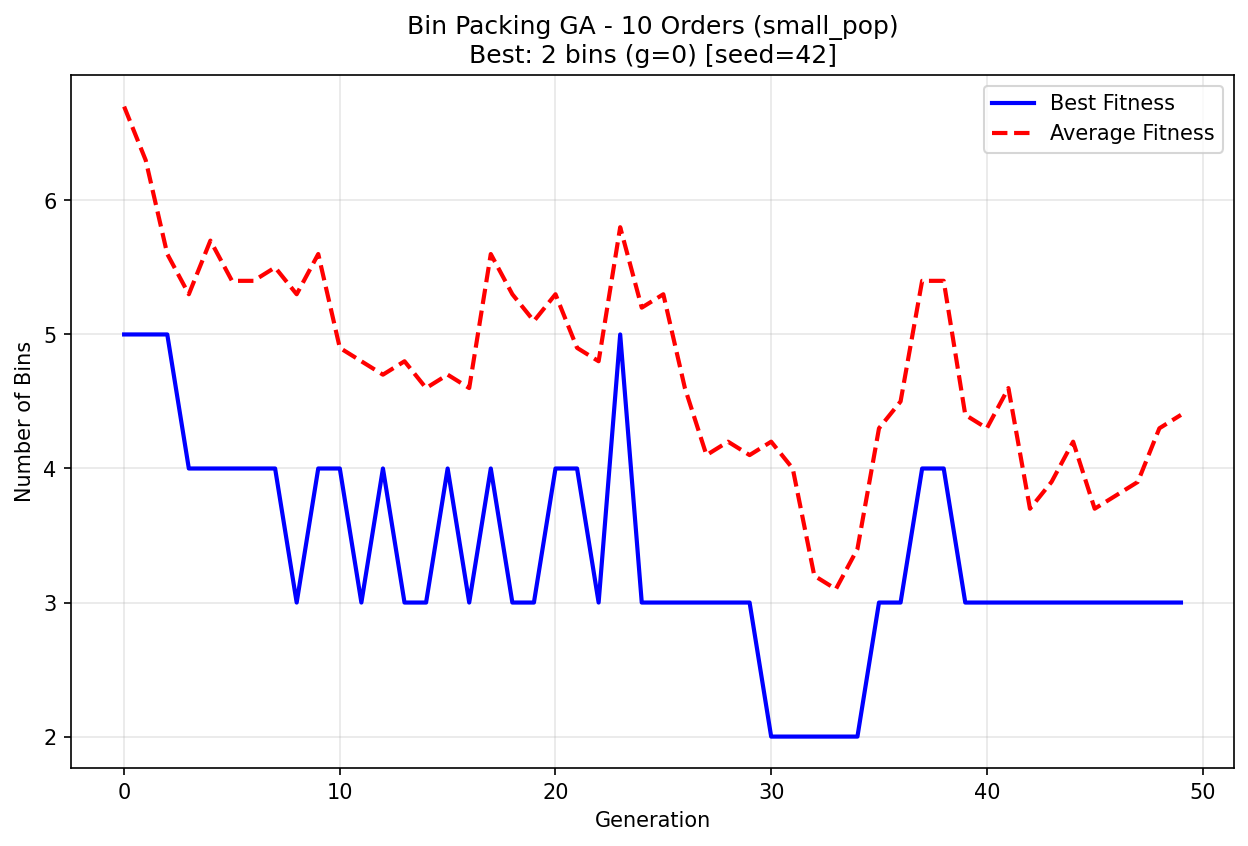
\includegraphics[width=\textwidth]{bpp_10items_small_pop_seed42.png}
    \caption{Small population: 10 orders}
    \label{fig:small_pop_10}
\end{minipage}\hfill
\begin{minipage}{0.48\textwidth}
    \centering
    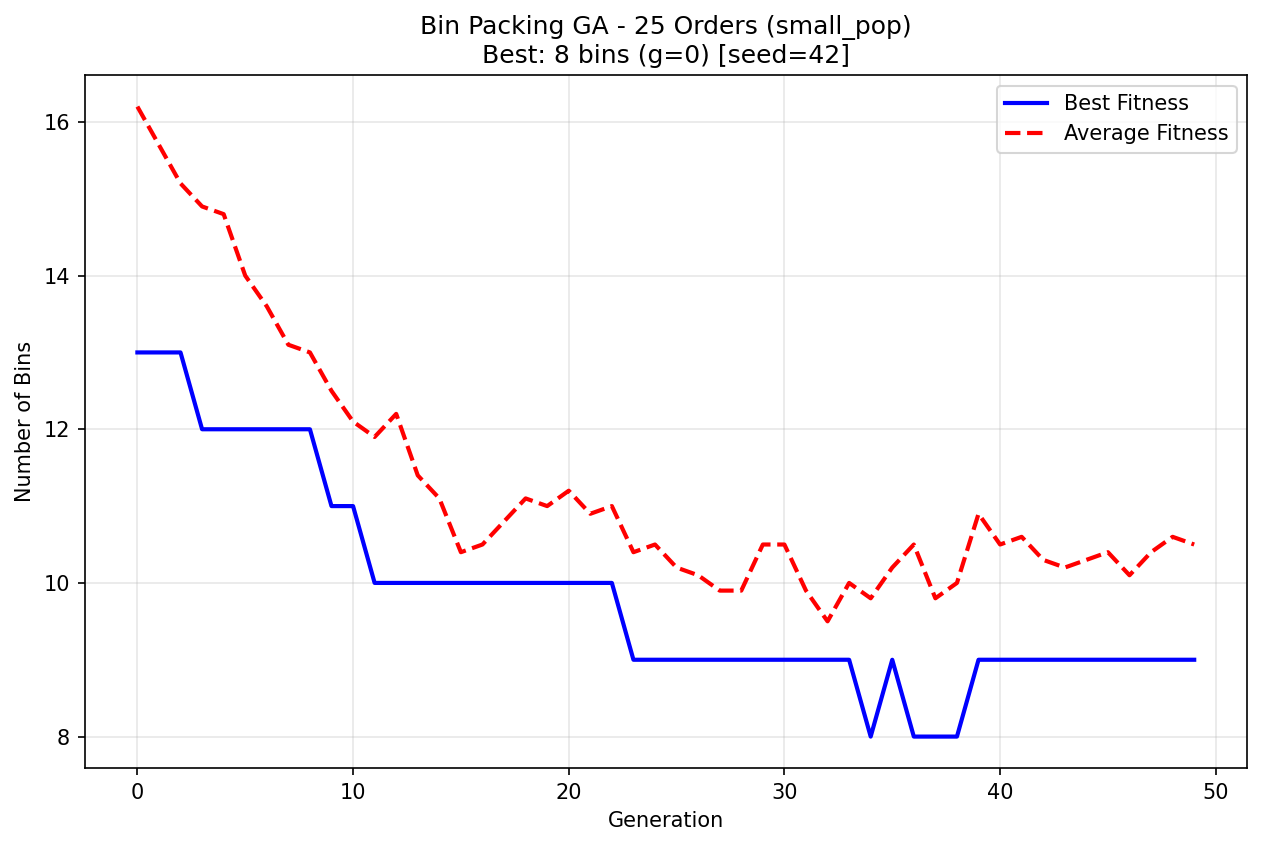
\includegraphics[width=\textwidth]{bpp_25items_small_pop_seed42.png}
    \caption{Small population: 25 orders}
    \label{fig:small_pop_25}
\end{minipage}
\end{figure}

\begin{figure}[htbp]
\begin{minipage}{0.48\textwidth}
    \centering
    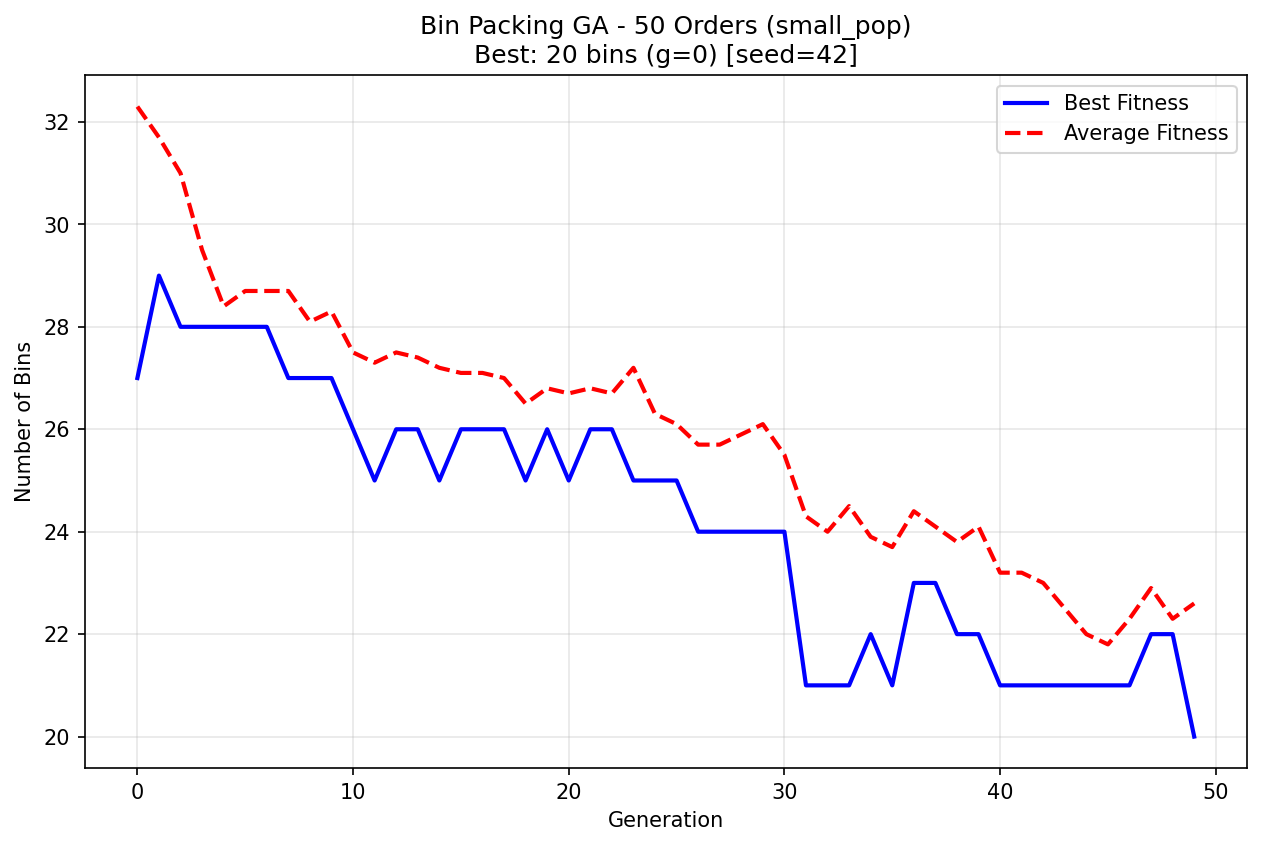
\includegraphics[width=\textwidth]{bpp_50items_small_pop_seed42.png}
    \caption{Small population: 50 orders}
    \label{fig:small_pop_50}
\end{minipage}\hfill
\begin{minipage}{0.48\textwidth}
    \centering
    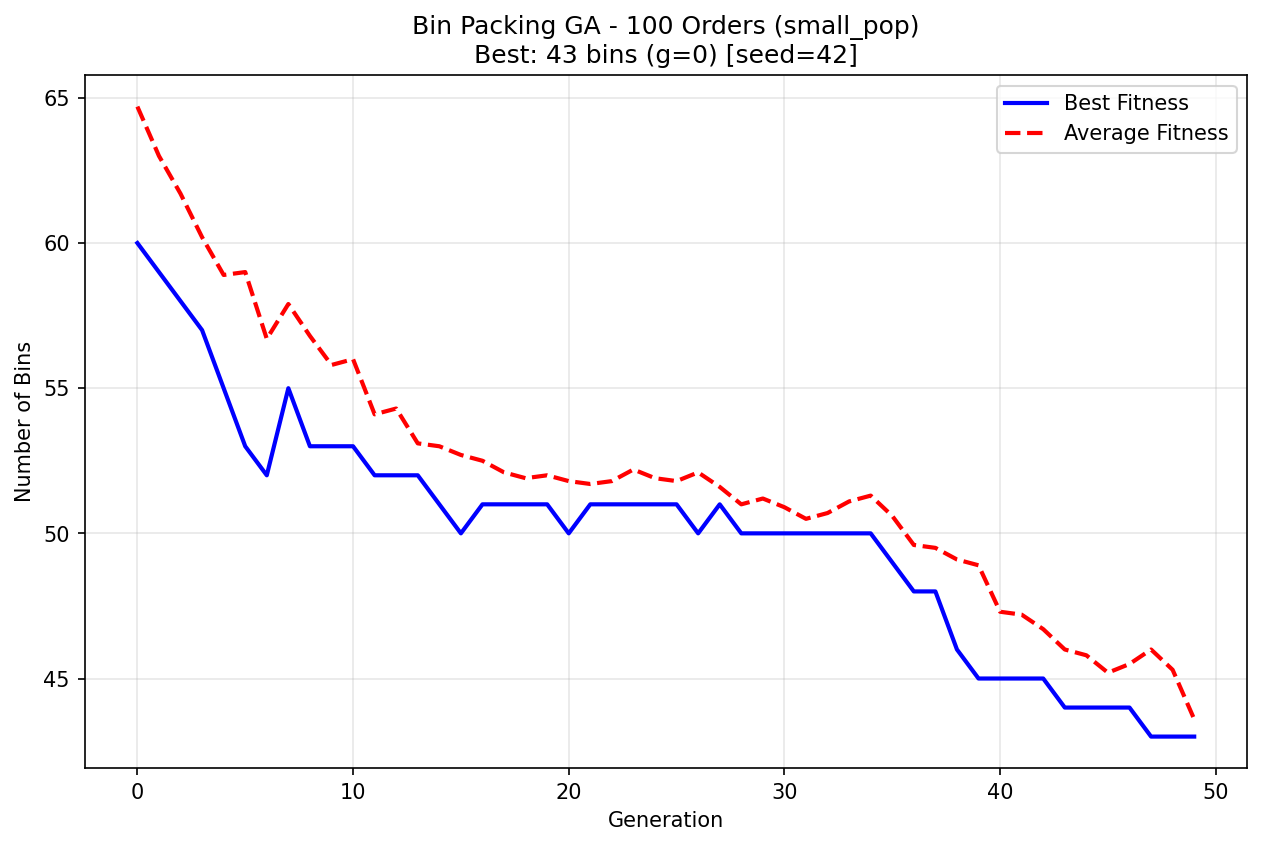
\includegraphics[width=\textwidth]{bpp_100items_small_pop_seed42.png}
    \caption{Small population: 100 orders}
    \label{fig:small_pop_100}
\end{minipage}
\end{figure}

% Large population
\begin{figure}[htbp]
\begin{minipage}{0.48\textwidth}
    \centering
    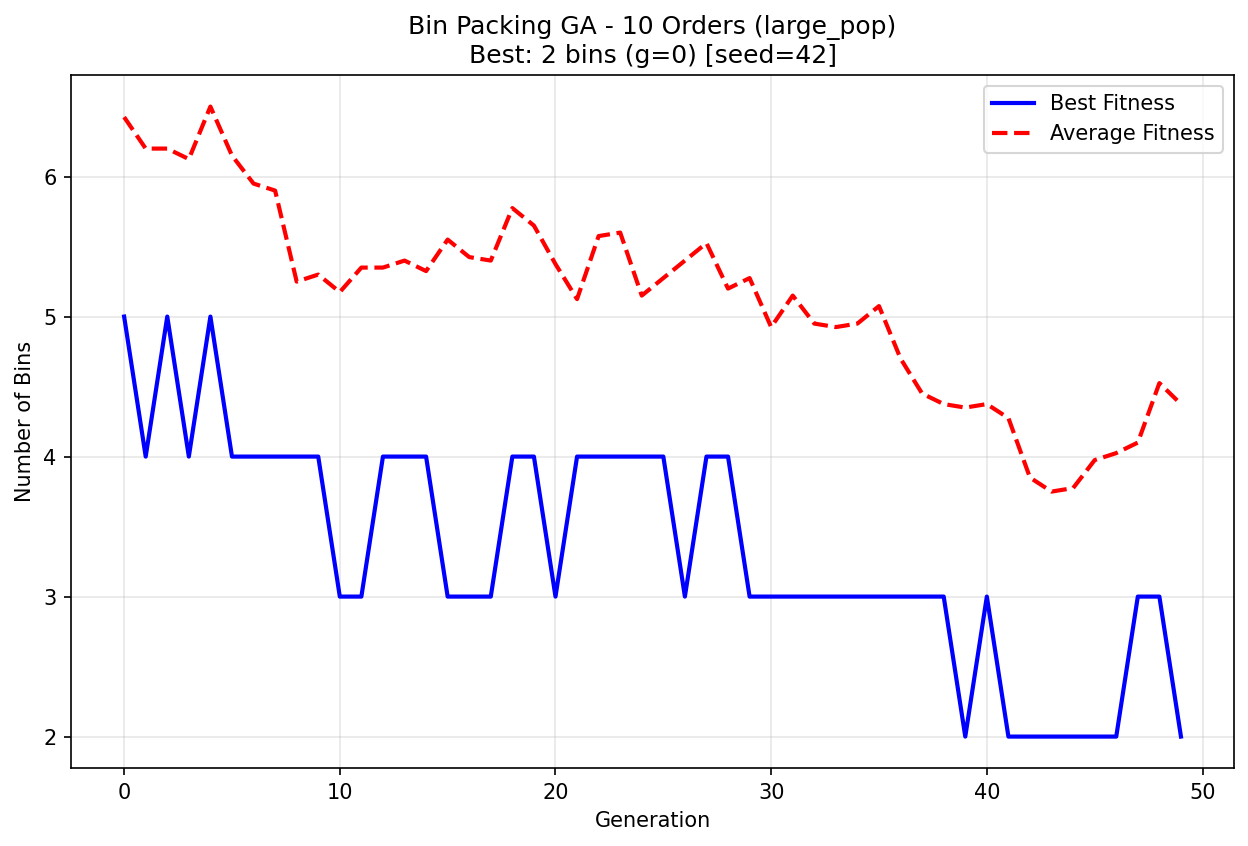
\includegraphics[width=\textwidth]{bpp_10items_large_pop_seed42.png}
    \caption{Large population: 10 orders}
    \label{fig:large_pop_10}
\end{minipage}\hfill
\begin{minipage}{0.48\textwidth}
    \centering
    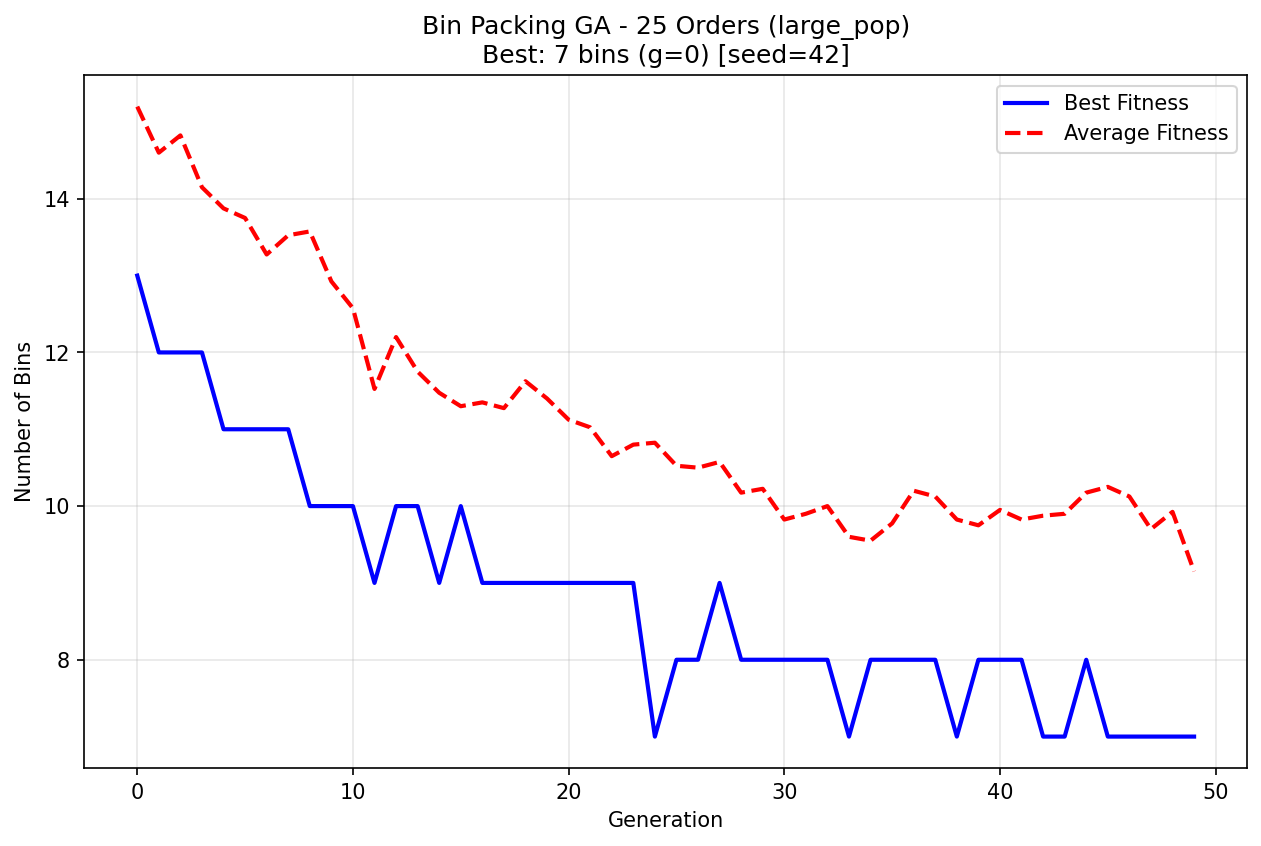
\includegraphics[width=\textwidth]{bpp_25items_large_pop_seed42.png}
    \caption{Large population: 25 orders}
    \label{fig:large_pop_25}
\end{minipage}
\end{figure}

\begin{figure}[htbp]
\begin{minipage}{0.48\textwidth}
    \centering
    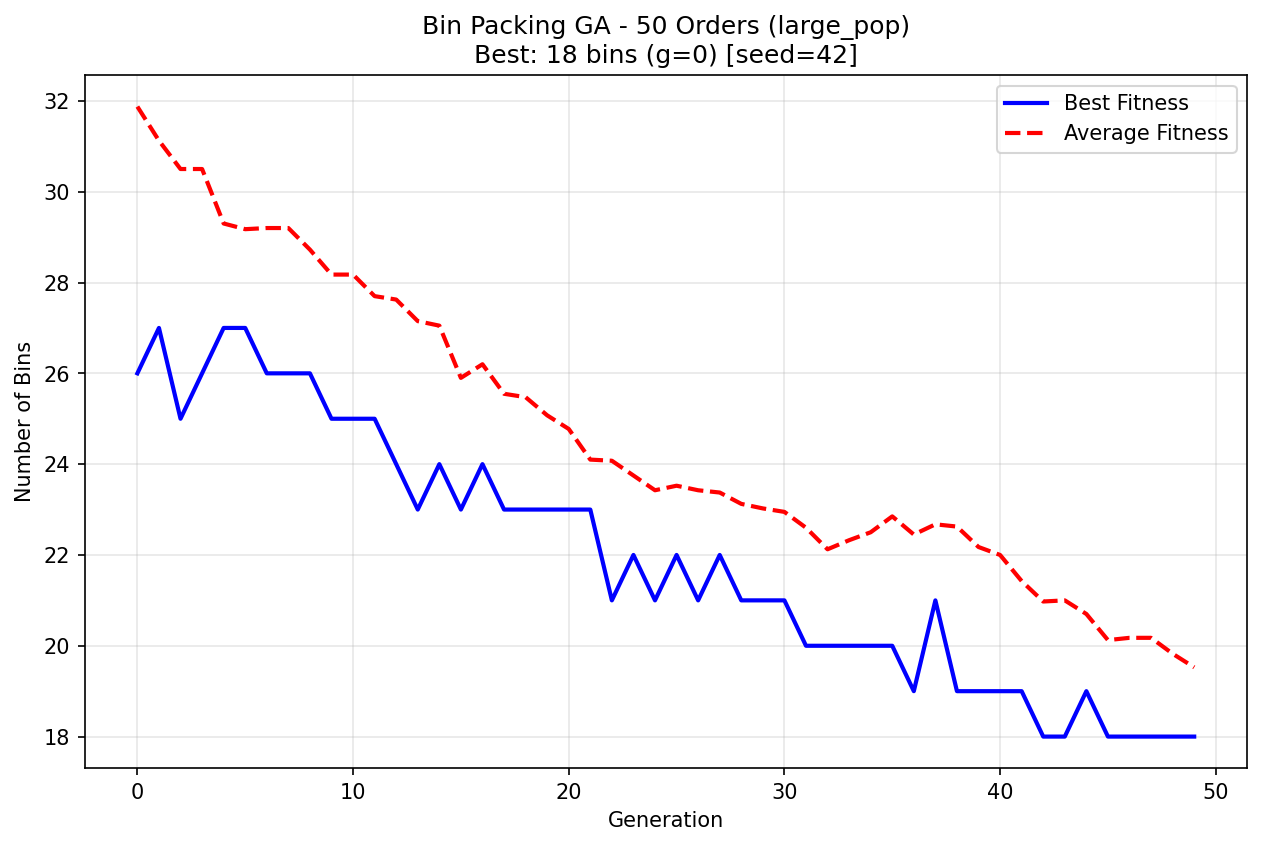
\includegraphics[width=\textwidth]{bpp_50items_large_pop_seed42.png}
    \caption{Large population: 50 orders}
    \label{fig:large_pop_50}
\end{minipage}\hfill
\begin{minipage}{0.48\textwidth}
    \centering
    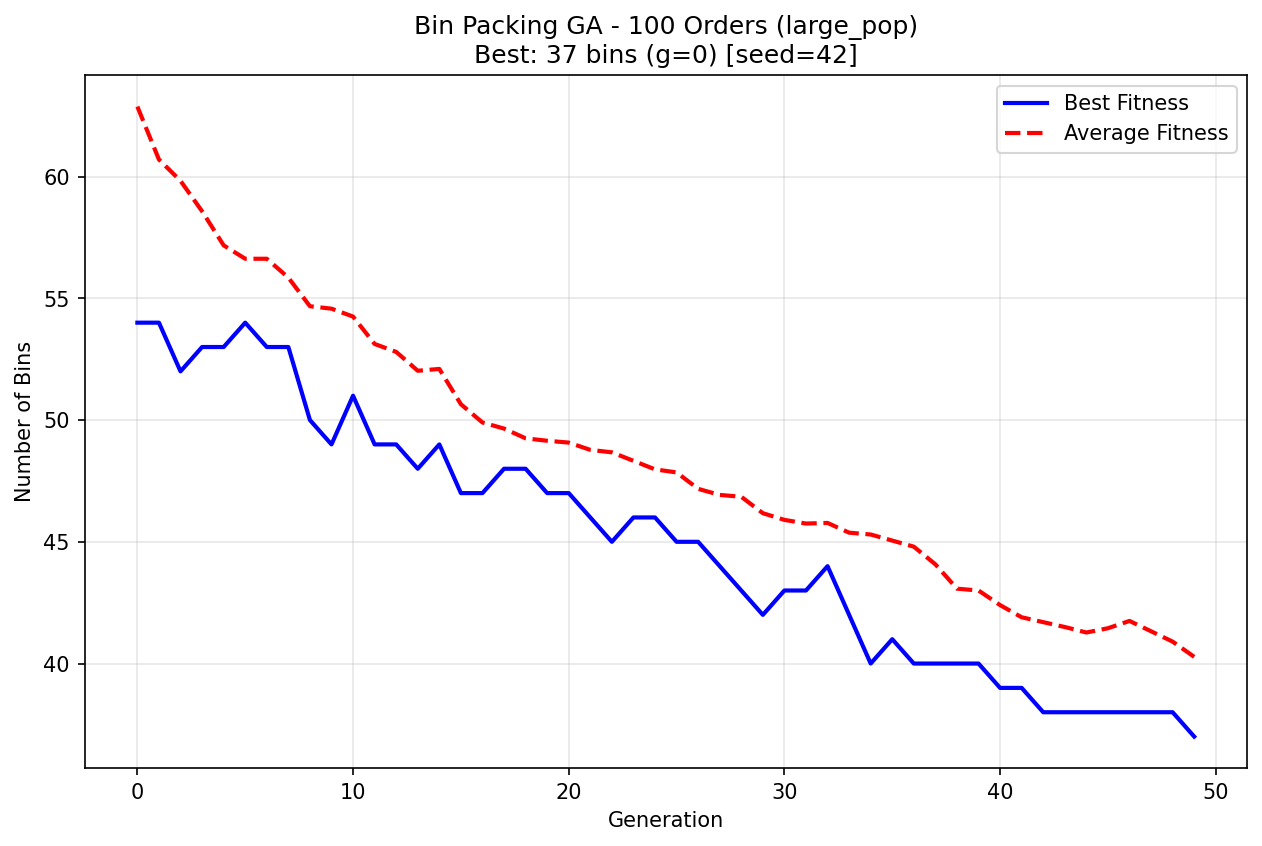
\includegraphics[width=\textwidth]{bpp_100items_large_pop_seed42.png}
    \caption{Large population: 100 orders}
    \label{fig:large_pop_100}
\end{minipage}
\end{figure}

% Short run
\begin{figure}[htbp]
\begin{minipage}{0.48\textwidth}
    \centering
    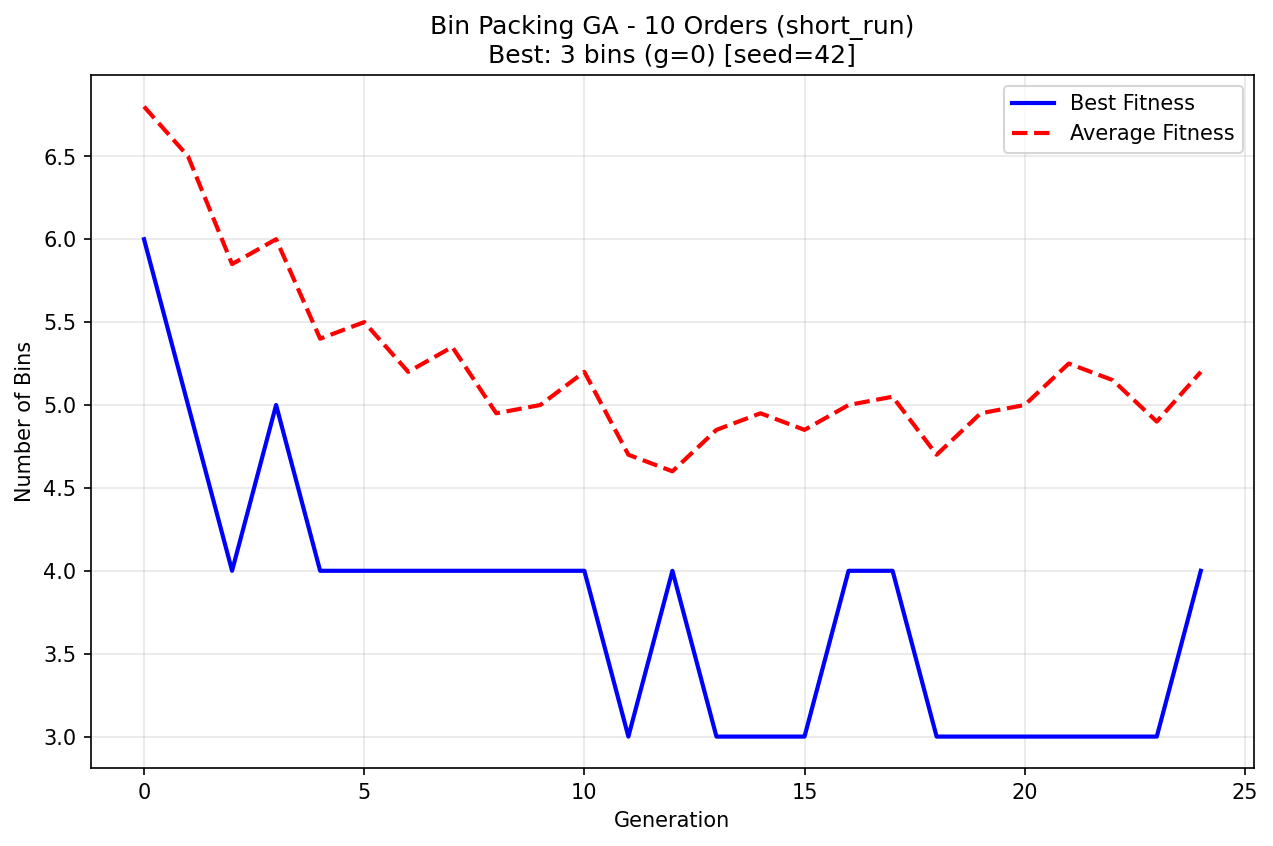
\includegraphics[width=\textwidth]{bpp_10items_short_run_seed42.png}
    \caption{Short run: 10 orders}
    \label{fig:short_run_10}
\end{minipage}\hfill
\begin{minipage}{0.48\textwidth}
    \centering
    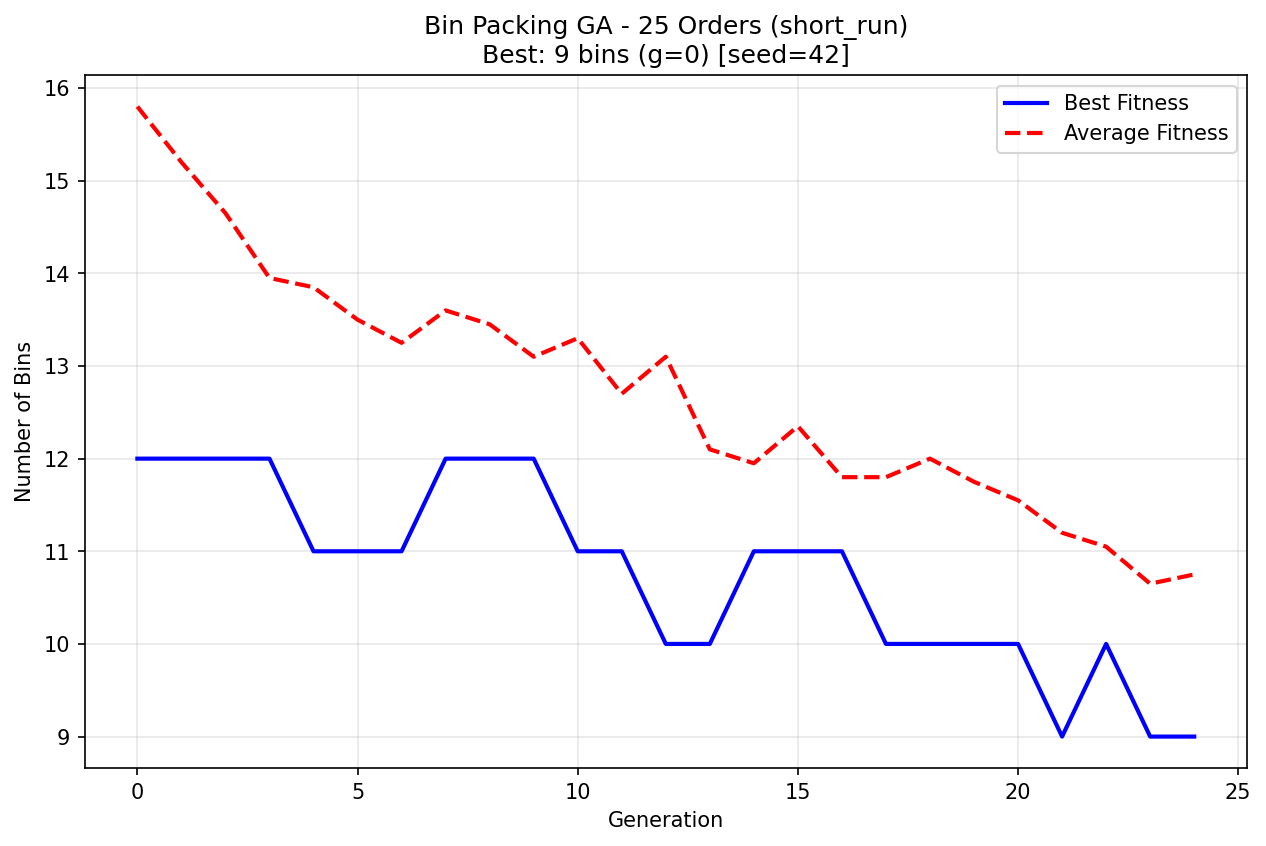
\includegraphics[width=\textwidth]{bpp_25items_short_run_seed42.png}
    \caption{Short run: 25 orders}
    \label{fig:short_run_25}
\end{minipage}
\end{figure}

\begin{figure}[htbp]
\begin{minipage}{0.48\textwidth}
    \centering
    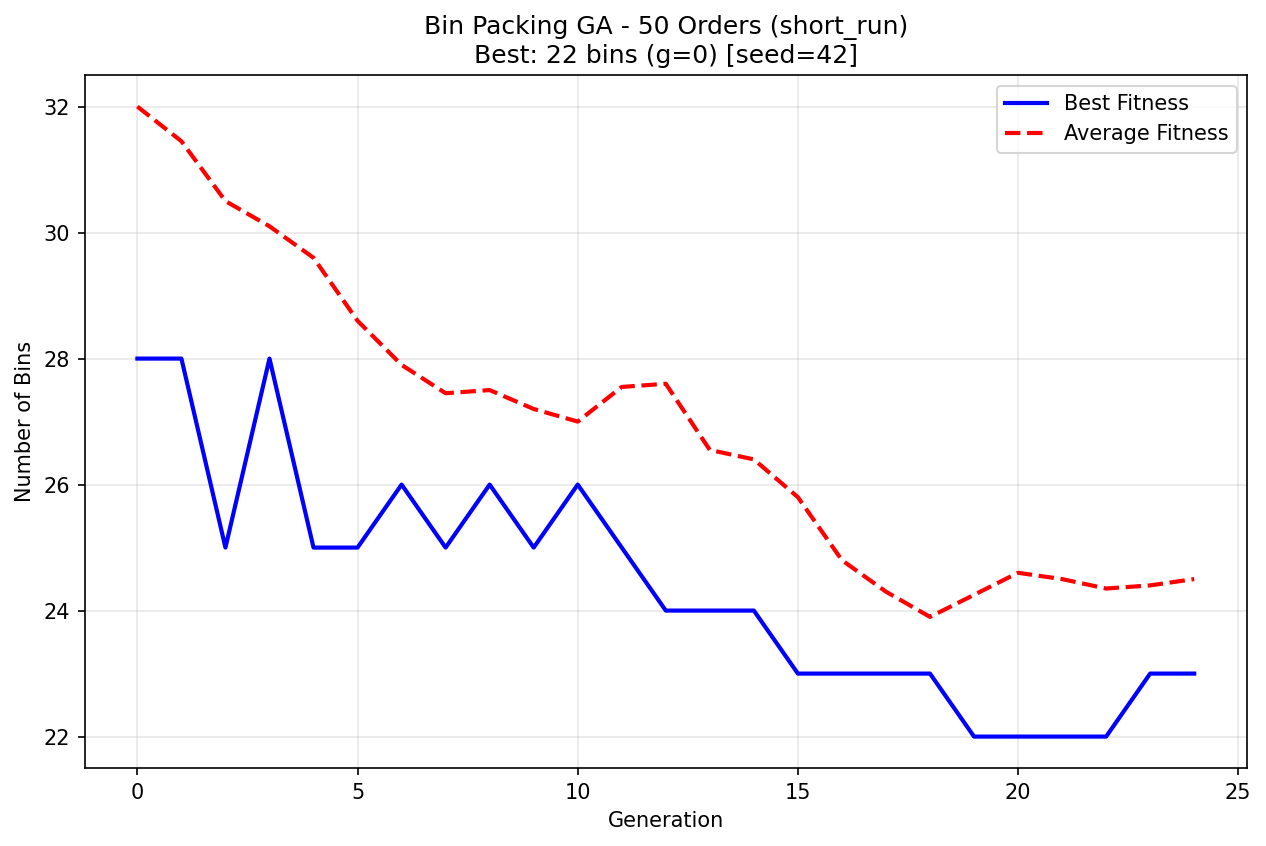
\includegraphics[width=\textwidth]{bpp_50items_short_run_seed42.png}
    \caption{Short run: 50 orders}
    \label{fig:short_run_50}
\end{minipage}\hfill
\begin{minipage}{0.48\textwidth}
    \centering
    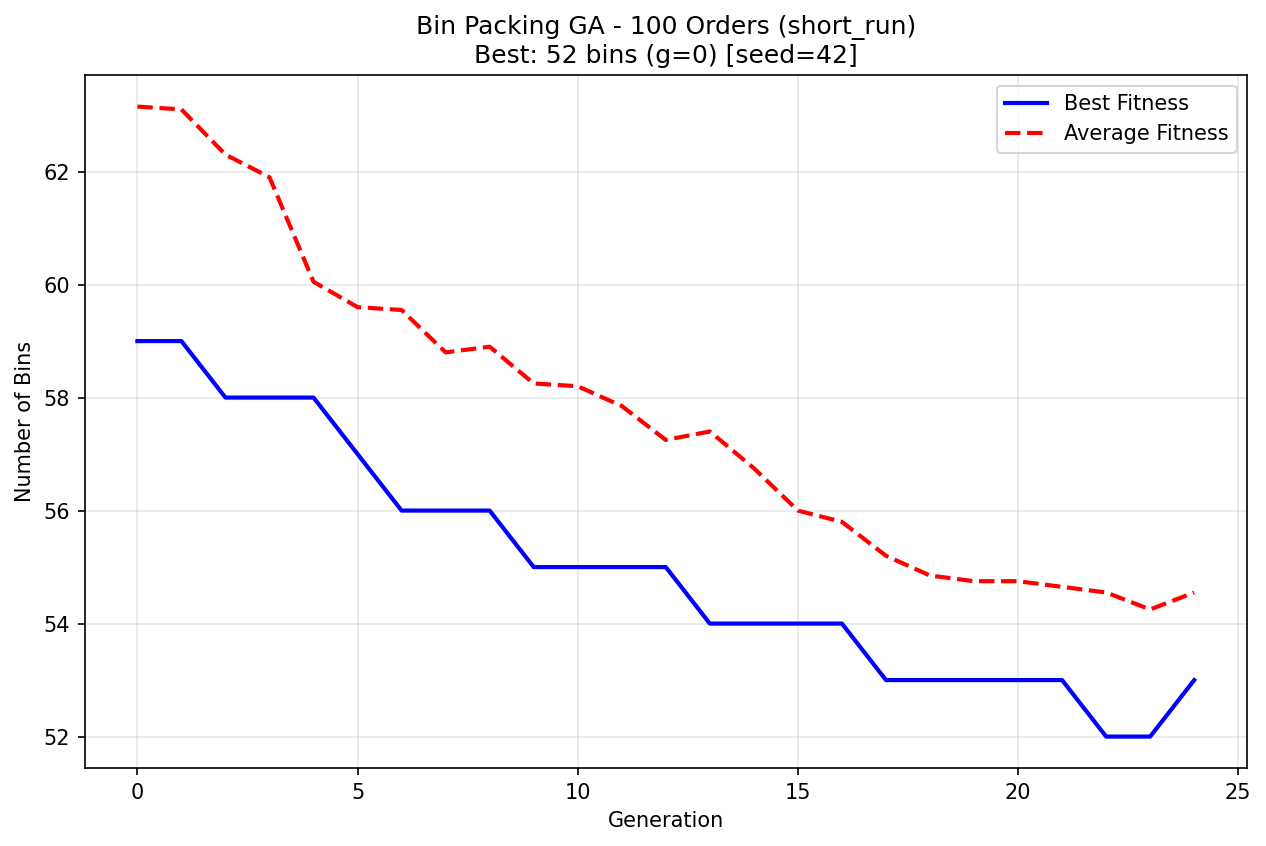
\includegraphics[width=\textwidth]{bpp_100items_short_run_seed42.png}
    \caption{Short run: 100 orders}
    \label{fig:short_run_100}
\end{minipage}
\end{figure}

% Long run
\begin{figure}[htbp]
\begin{minipage}{0.48\textwidth}
    \centering
    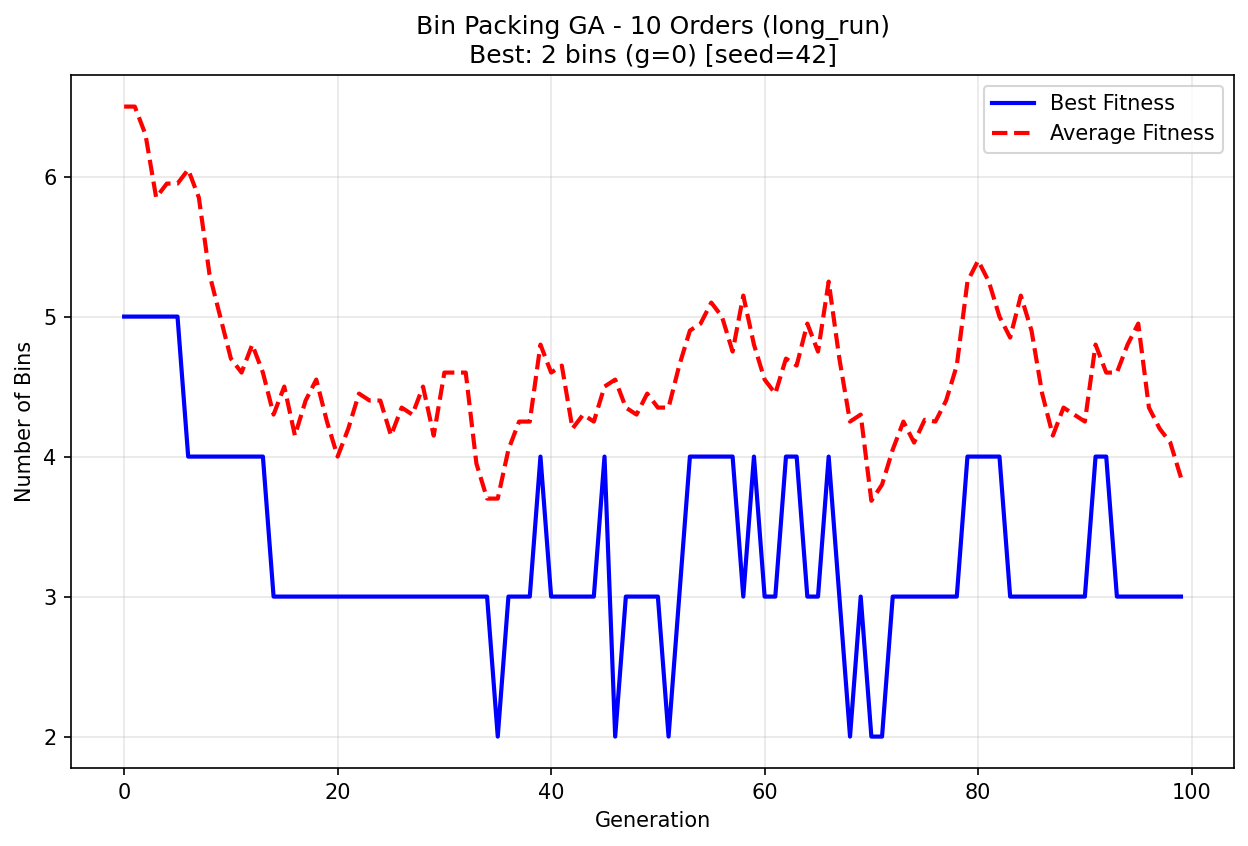
\includegraphics[width=\textwidth]{bpp_10items_long_run_seed42.png}
    \caption{Long run: 10 orders}
    \label{fig:long_run_10}
\end{minipage}\hfill
\begin{minipage}{0.48\textwidth}
    \centering
    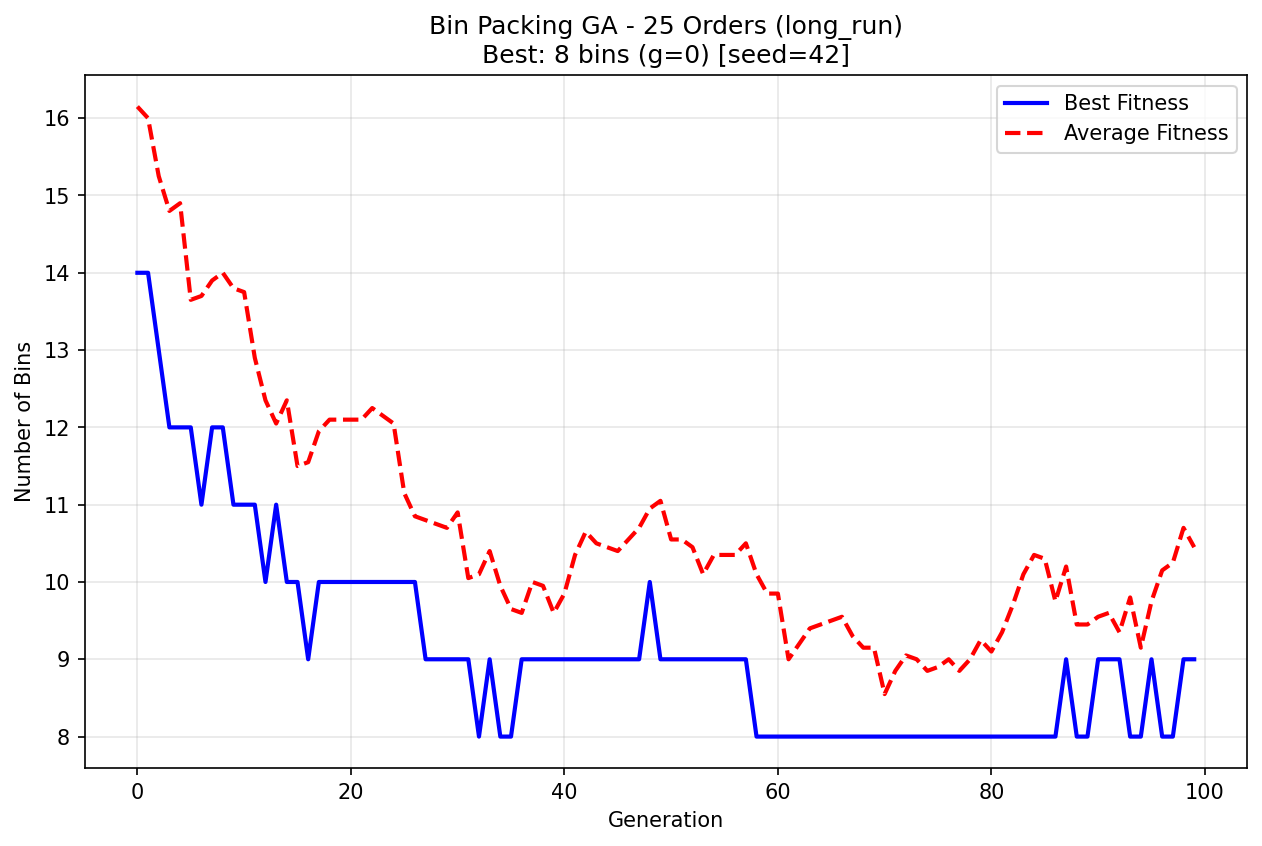
\includegraphics[width=\textwidth]{bpp_25items_long_run_seed42.png}
    \caption{Long run: 25 orders}
    \label{fig:long_run_25}
\end{minipage}
\end{figure}

\begin{figure}[htbp]
\begin{minipage}{0.48\textwidth}
    \centering
    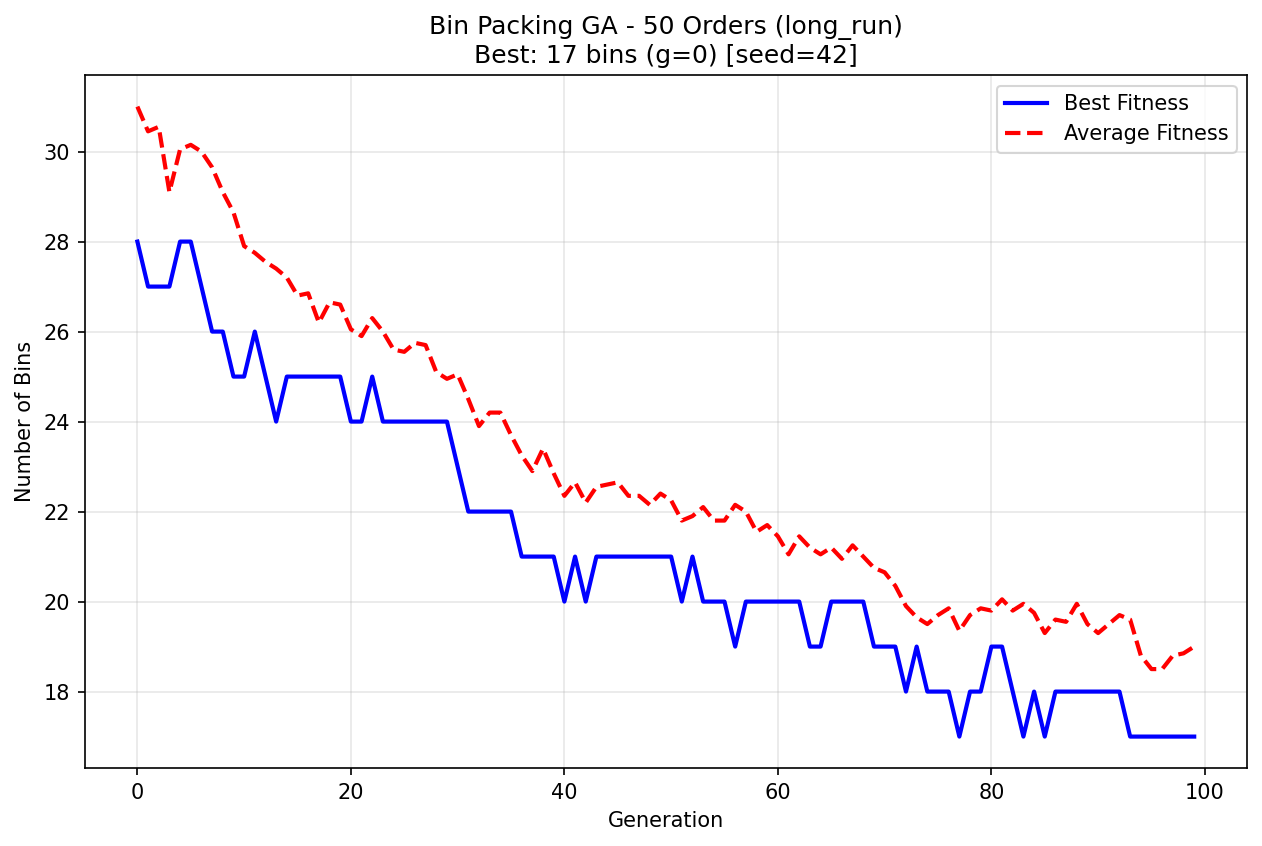
\includegraphics[width=\textwidth]{bpp_50items_long_run_seed42.png}
    \caption{Long run: 50 orders}
    \label{fig:long_run_50}
\end{minipage}\hfill
\begin{minipage}{0.48\textwidth}
    \centering
    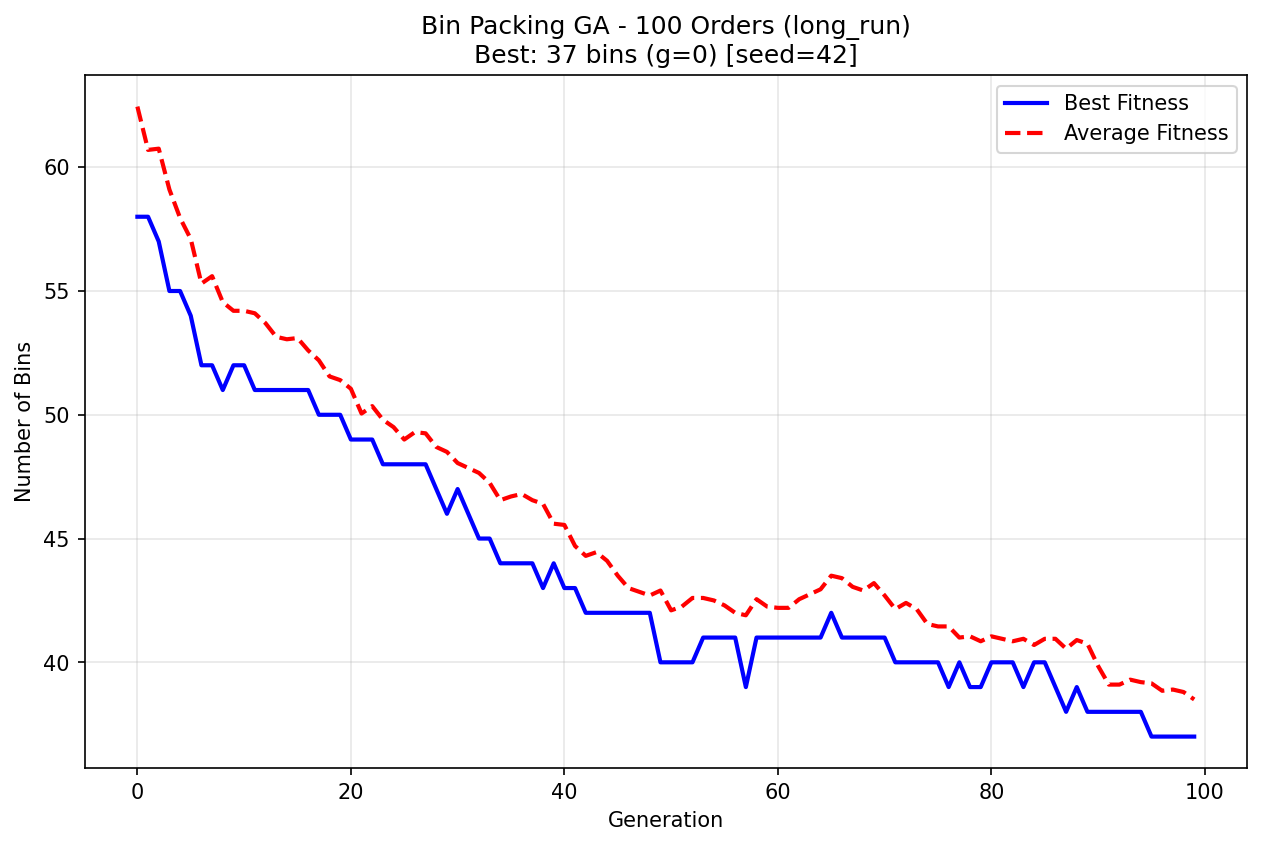
\includegraphics[width=\textwidth]{bpp_100items_long_run_seed42.png}
    \caption{Long run: 100 orders}
    \label{fig:long_run_100}
\end{minipage}
\end{figure}

\subsection{Best Solutions}

Report the best solution found and its bin-wise packing configuration.

\section{Q5: Analysis and Comparison}

\subsection{Convergence Analysis}

Compare the convergence behavior of different runs (e.g., different random seeds or order sizes).

\subsection{Performance Comparison}

Discuss whether the algorithm tends to find feasible solutions early or late in the process.

\section{Conclusion}
This study successfully implemented...

\end{document}